% =====================================================================================
% Chapter 5 - TriMVPP version (seven final checkpoints, FP16, Integrated Gradients + attention, measured latency)
% Required packages in the preamble: graphicx, booktabs, amsmath.
% Figures: copy the folder Demo/docs/figures into the thesis project as figures/.
% =====================================================================================

\chapter{SYSTEM DESIGN AND IMPLEMENTATION}
\label{chap:system_design}

This chapter describes how the TriMVPP framework presented in Chapter~4 is implemented as an interactive web-based system. It covers the system architecture, the integration of foundation models and bioinformatics resources, the single-variant and batch workflows, data management and deployment, the web interface, and the system's response time.

% -------------------------------------------------------------------------------------
\section{System Architecture}
\label{sec:system_architecture}

The system follows a three-tier client--server architecture (Fig.~\ref{fig:system_architecture}) that separates user interaction, AI processing, and data management, so that heavy annotation and inference tasks do not block the user interface. The React frontend communicates with a FastAPI backend through REST for single-variant queries and Server-Sent Events (SSE) for streaming batch results. The backend manages the complete inference workflow and runs long operations, such as VEP annotation and GPU computation, in background threads. All data resources, including the PostgreSQL database and the bioinformatics references, are deployed locally, which keeps annotation results consistent and means that the system does not depend on external web services.

The presentation tier is a single-page application that keeps its state in the browser: the selected variant and feature configuration are stored in the URL so that a result can be shared or reopened, and batch progress is kept in session storage so that it is not lost when the user changes pages. The application tier checks the format of every request and response and gives each request an ID, which is used for logging and for measuring the time of each stage. The data tier combines a relational database, which stores variants, features, and predictions, with read-only reference resources: the GRCh38 genome and Ensembl proteome, the SpliceAI archive, and two FAISS indexes, each containing the $23{,}208$ training-set embedding displacements of one foundation model.

\begin{figure}[htbp]
    \centering
    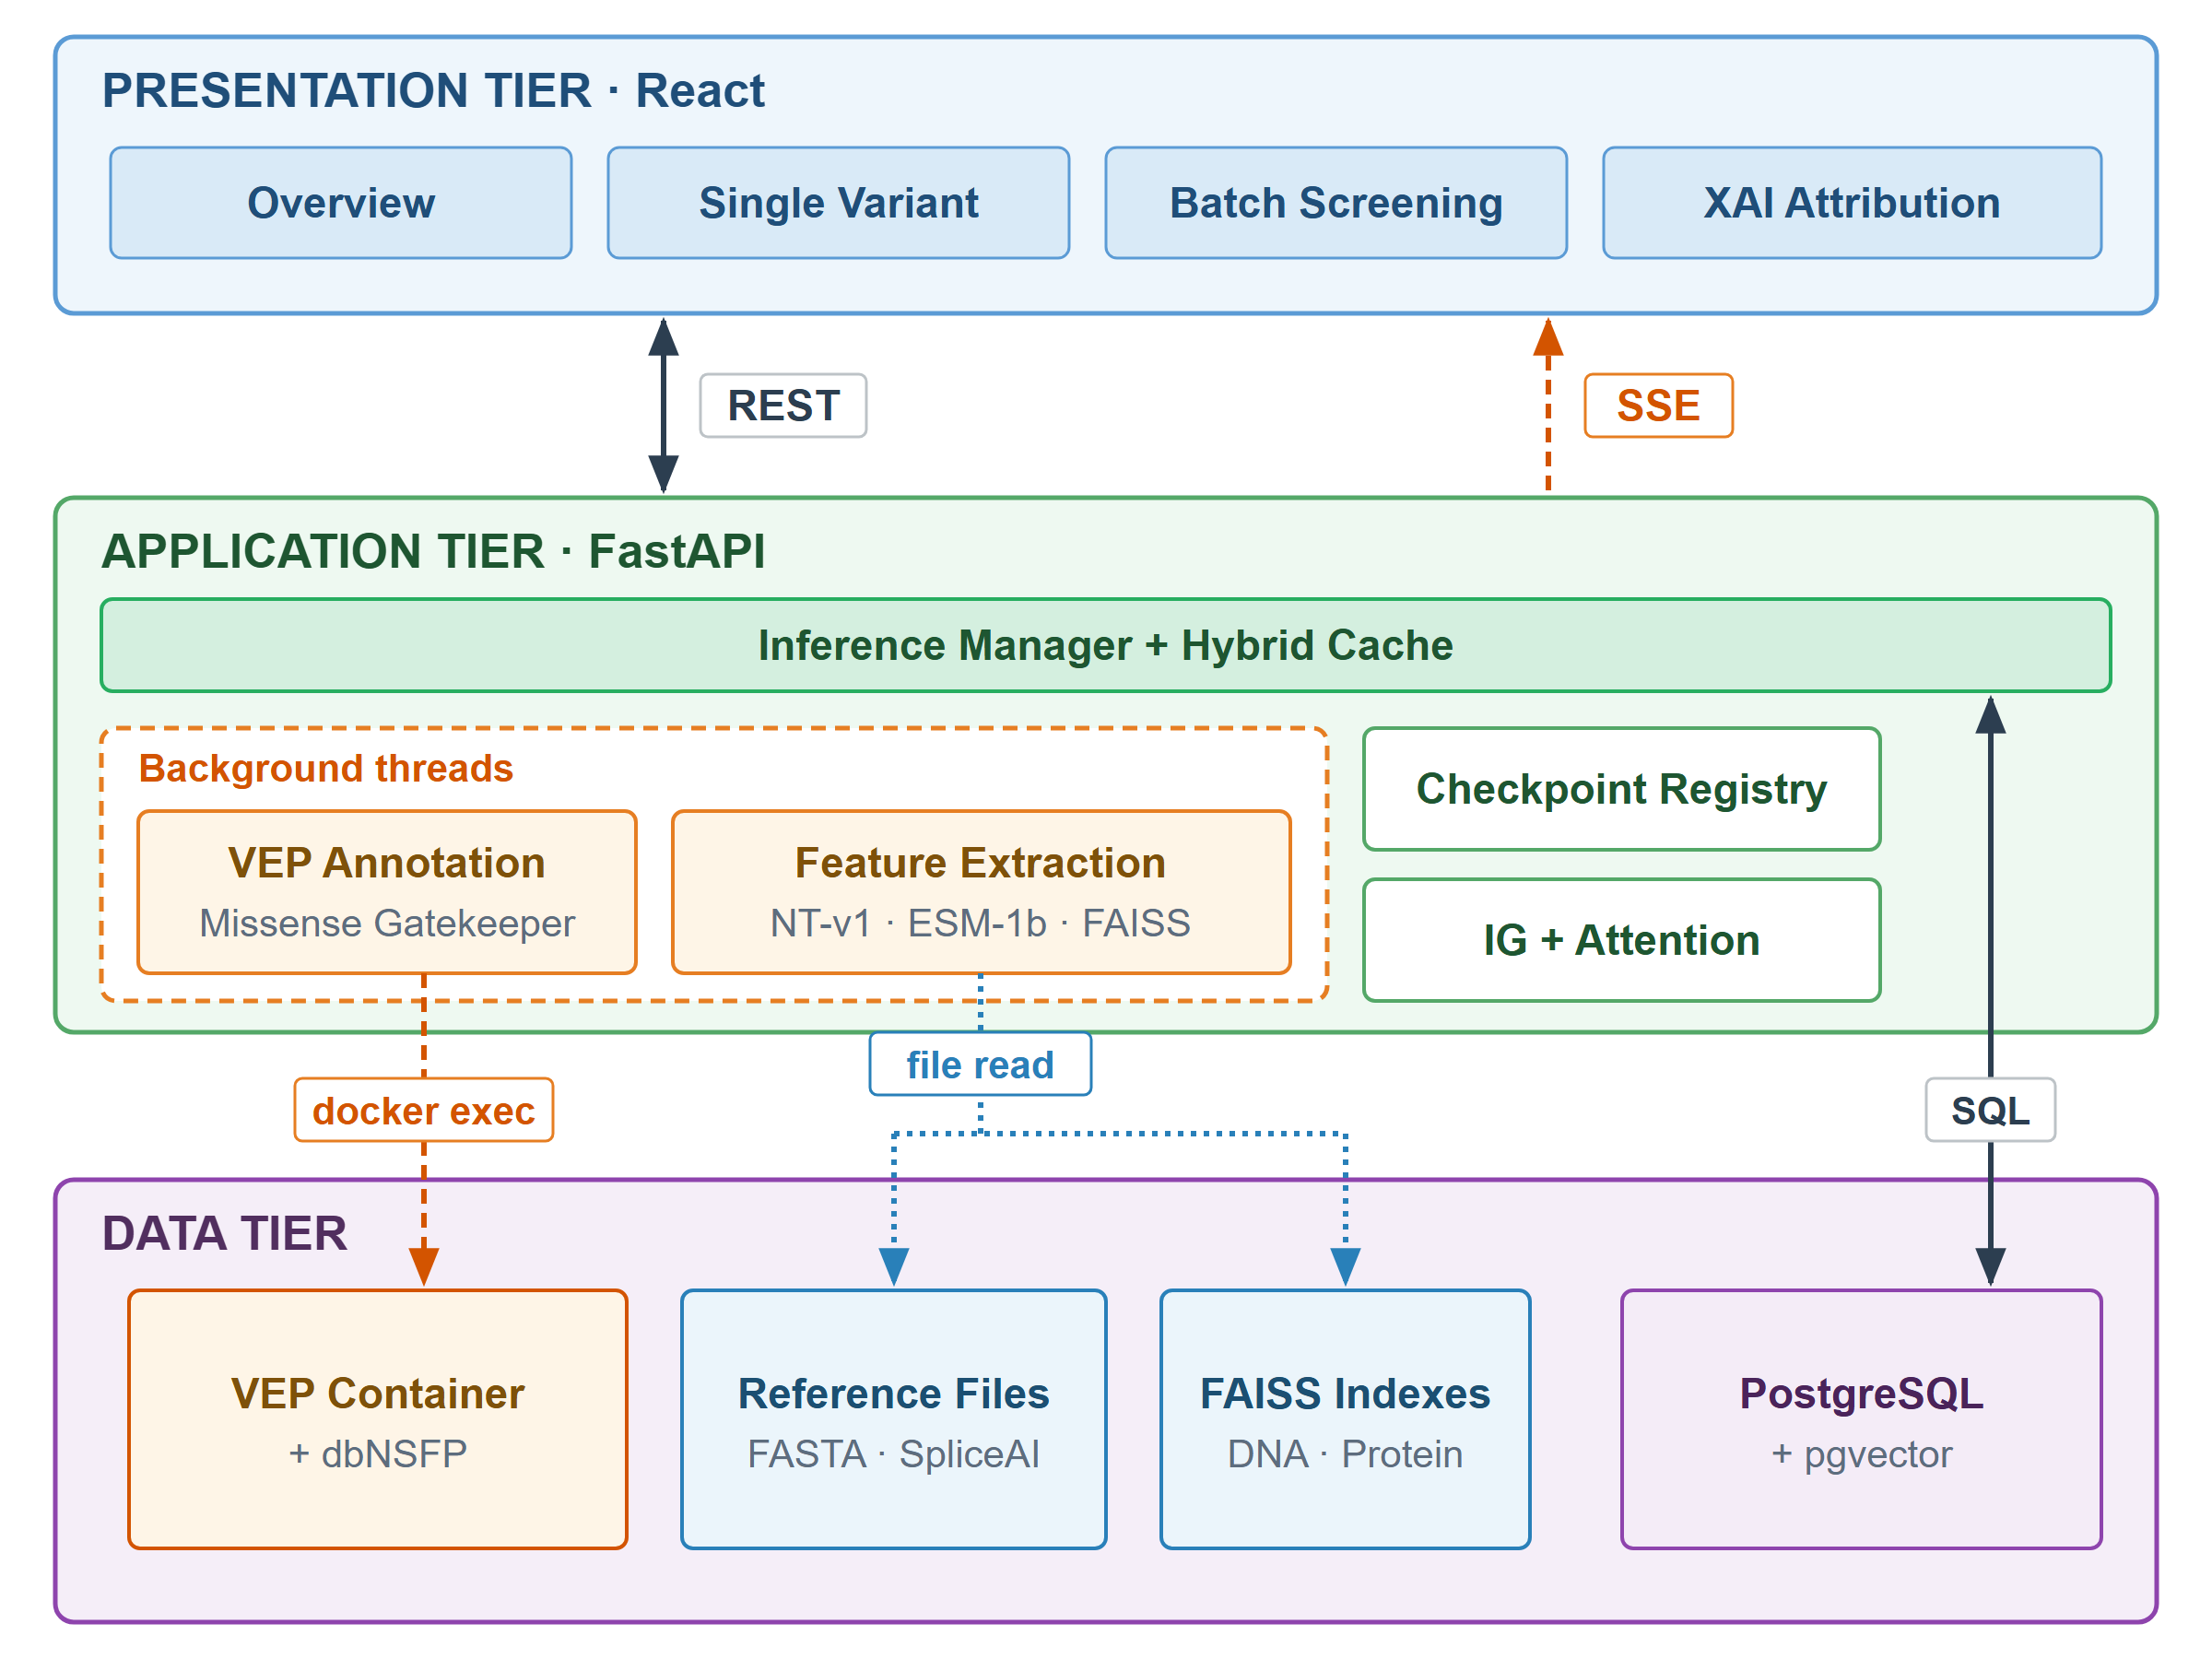
\includegraphics[width=0.95\textwidth]{figures/5.1.png}
    \caption{Three-tier architecture of the TriMVPP system.}
    \label{fig:system_architecture}
\end{figure}

% -------------------------------------------------------------------------------------
\section{Artificial Intelligence Model and Bioinformatics Integration}
\label{sec:ai_integration}

\subsection{Feature Extraction Pipeline}

To avoid a long delay on the first request, the backend loads the foundation models, sequence and FAISS indexes, and normalization files once at startup and performs a warm-up forward pass before accepting requests. Each variant, specified as \texttt{chr:pos:ref>alt} on GRCh38, is annotated by the offline Ensembl VEP service, which selects the MANE Select or canonical transcript and provides the consequence, the protein position, and the eleven core biological features: two population allele frequencies from the VEP cache and nine conservation scores from dbNSFP. AlphaMissense, REVEL, and ClinVar annotations are collected at the same time for comparison.

Since TriMVPP is trained only on missense single-nucleotide variants, a missense gatekeeper rejects all other consequence types, and the reference allele and amino acid are checked against the local GRCh38 genome and proteome to detect inputs from a wrong genome build. For accepted variants, the nine SpliceAI features are read from the compressed SpliceAI archive through a custom tabix reader that decompresses only the blocks surrounding the variant. The DNA and protein windows ($1{,}001$~bp and $501$~aa) centered on the mutation are encoded by NT-v1 500M\footnote{\url{https://huggingface.co/InstaDeepAI/nucleotide-transformer-500m-human-ref}} and ESM-1b 650M\footnote{\url{https://huggingface.co/facebook/esm1b_t33_650M_UR50S}} in FP16 precision, as in training. From the last hidden layer of each model, the system keeps a window of $33$ tokens centered on the variant ($16$ on each side) for both the reference and the alternative sequence, which forms the sequence input of TriMVPP. The embeddings of the central token are used to compute the geometric descriptors. For each foundation model, four descriptors are calculated: the Euclidean and cosine distances between the reference and alternative embeddings, the Euclidean distance relative to the norm of the reference embedding, and the local intrinsic dimensionality of the embedding displacement, estimated from its $k = 64$ nearest neighbors in the corresponding FAISS index. Table~\ref{tab:tabular_features} lists the resulting $28$ tabular features, which are standardized with the imputers and scalers fitted on the training set.

\begin{table}[htbp]
    \centering
    \caption{Tabular features extracted for each variant.}
    \label{tab:tabular_features}
    \begin{tabular}{lp{0.54\textwidth}c}
        \toprule
        \textbf{Group} & \textbf{Features} & \textbf{Count} \\
        \midrule
        Allele frequency & 1000 Genomes and gnomAD exomes & 2 \\
        Conservation & Three phyloP, three phastCons, and three GERP-based scores & 9 \\
        SpliceAI & Four delta scores, four delta positions, and the maximum delta score & 9 \\
        Geometry & Four descriptors for each of the DNA and protein central-token embeddings & 8 \\
        \midrule
        Total & & 28 \\
        \bottomrule
    \end{tabular}
\end{table}

\subsection{Ablation-Aware Model Routing}

The web interface provides three feature groups, each controlled by a single switch: \textit{DNA}, \textit{Protein}, and \textit{Bio + Geom + SpliceAI}. Since disabling all groups is not allowed, the system supports seven configurations (Table~\ref{tab:ablation_configs}). Each configuration has its own separately trained TriMVPP checkpoint: the branches of a disabled group are removed from the network rather than filled with zeros, and cross-attention is applied only when at least two branches are active. A checkpoint registry links each configuration to its checkpoint, builds the matching branches, and loads the weights only if all parameter names and shapes match exactly. Each checkpoint uses the threshold $\tau$ that maximizes MCC on the validation set, and a variant is classified as \textit{Pathogenic} if $p \geq \tau$ and as \textit{Benign} otherwise. The biological, geometric, and SpliceAI features share one switch, so that they are always enabled or disabled together.

\begin{table}[htbp]
    \centering
    \caption{Feature-ablation configurations supported by the checkpoint registry.}
    \label{tab:ablation_configs}
    \begin{tabular}{clrcc}
        \toprule
        \textbf{Key} & \textbf{Active feature groups} & \textbf{Parameters} & $\boldsymbol{\tau}$ & \textbf{Attention maps} \\
        \midrule
        \texttt{111} & DNA, Protein, Bio + Geom + SpliceAI & 33,273,860 & 0.4791 & Yes \\
        \texttt{110} & DNA, Protein & 23,257,091 & 0.6340 & Yes \\
        \texttt{101} & DNA, Bio + Geom + SpliceAI & 21,908,483 & 0.7515 & Yes \\
        \texttt{011} & Protein, Bio + Geom + SpliceAI & 21,908,483 & 0.5660 & Yes \\
        \texttt{100} & DNA & 2,431,490 & 0.4819 & No \\
        \texttt{010} & Protein & 2,431,490 & 0.7383 & No \\
        \texttt{001} & Bio + Geom + SpliceAI & 1,082,882 & 0.6309 & No \\
        \bottomrule
    \end{tabular}
\end{table}

To check that the deployed pipeline reproduces the offline experiments, $440$ variants of the internal test set were processed by the complete web pipeline and compared with the predictions saved during evaluation. The mean absolute difference in probability was at most $0.0011$ for every configuration, and the predicted labels were identical for five configurations, including the full one. The remaining two differed on two (\texttt{010}) and one (\texttt{001}) variants whose probabilities lie close to the threshold.

\subsection{Integrated Explainability}

Each prediction is explained with two complementary methods, following the explainability analysis of the trained models: Integrated Gradients (IG)~\cite{sundararajan2017axiomatic}, which measures how much each input contributes to the prediction, and the attention maps of the cross-attention layers, which show how information flows between the branches.

IG explains the Pathogenic logit $f(\mathbf{x})$, that is, the model output before the sigmoid, with respect to all inputs of the active branches: the DNA and protein token windows (reference and alternative, $33 \times 1{,}280$ values each) and the $20$ biological and SpliceAI and $8$ geometric standardized features. Each input is compared with a baseline $\mathbf{x}'$, and the gradient of the logit is integrated along the straight path from $\mathbf{x}'$ to $\mathbf{x}$:
\[
    \mathrm{IG}_i(\mathbf{x}) = (x_i - x'_i) \int_{0}^{1} \frac{\partial f\big(\mathbf{x}' + \alpha (\mathbf{x} - \mathbf{x}')\big)}{\partial x_i}\, d\alpha .
\]
The baseline is fixed and shared by all requests. It consists of the mean token windows and the median tabular features of $256$ variants randomly sampled from the training set, so the explanation of a variant does not depend on which or how many variants the user submits. The integral is approximated with the trapezoidal rule over $64$ steps, evaluated on the GPU in FP32 in groups of eight interpolation points. IG satisfies the completeness property
\[
    \sum_{i} \mathrm{IG}_i(\mathbf{x}) = f(\mathbf{x}) - f(\mathbf{x}'),
\]
so the remaining difference measures the approximation error. If it exceeds $5\%$ of $|f(\mathbf{x}) - f(\mathbf{x}')|$, the attributions are computed again with $128$ steps, and a warning is shown if the error is still larger. The attributions are then summed into three views: one value for each branch (DNA, Protein, Bio + SpliceAI, and Geometry), one value for each token position and allele (summed over the $1{,}280$ embedding dimensions), and one value for each tabular feature. IG is not part of the prediction request: it is computed the first time the explainability view of a prediction is opened and then stored with that prediction, so that later views reuse it. Single-variant and batch predictions are therefore not slowed down by the explanation.

The attention maps contain the weights of all three cross-attention layers and all eight heads. In each layer, every token of a query branch distributes its attention over the concatenated tokens of the other active branches, so each row of a map sums to one. Because the maps are large (about $1$~MB for the full configuration), they are computed only when the explainability view is opened, from the stored features, and are not saved in the database. The three single-branch configurations have no cross-attention layers and are explained by IG only. Attention weights describe where a branch reads information from, not how important that information is for the prediction, so the two methods are shown side by side.

To check the implementation, the explanations of $200$ test variants were computed with the web system for the full configuration and compared with the offline results of the same checkpoint. For this comparison, the eleven core biological features were taken from the stored test-set annotations, while all other inputs were extracted by the web pipeline. The median absolute difference in the logit was $0.001$ (maximum $0.038$), caused by small numerical differences in the re-extracted embeddings. The rankings of the attributions agreed almost perfectly, with Spearman correlations of at least $0.9998$ at the branch level, $0.9999$ at the feature level, and $1.000$ at the token level, and the most important feature was the same for all $200$ variants. The attention weights of $48$ variants differed by at most $0.0014$, and the largest completeness error was $1.7\%$ of the logit change.

% -------------------------------------------------------------------------------------
\section{Data Flow and Communication Protocols}
\label{sec:data_flow}

\subsection{Single-Variant Inference with Hybrid Lazy-Caching}

To keep the system fast for interactive use, extracted features and predictions are cached separately, so that each request follows one of the three paths in Fig.~\ref{fig:single_sequence}.

\begin{itemize}
    \item \textit{Cache hit:} a valid prediction exists for the variant and the selected configuration, and it is returned directly from the database.
    \item \textit{Feature reuse:} valid features exist, but the prediction must be recomputed because the user changed the feature configuration, enabled \textit{Live Bypass}, or the checkpoint was updated. The stored token windows and unscaled features are reloaded, and only normalization and classification are executed again.
    \item \textit{Cache miss:} no valid features exist, and the full pipeline is executed.
\end{itemize}

On a cache miss, the variant is first annotated by VEP and must pass the missense gatekeeper before any feature is extracted, so rejected variants use neither the GPU nor the SpliceAI archive. Only then are the DNA and protein windows built, using the protein isoform and residue position provided by VEP, encoded by NT-v1 and ESM-1b, and the SpliceAI scores read. The extracted features are saved before classification, so that the slow extraction does not need to be repeated if a later step fails.

Cached results are given a version to avoid using outdated data. Features are stored with a hash of the extraction settings, such as the foundation model names, sequence and token window lengths, compute device, and numerical precision, while predictions also store the name and modification time of the checkpoint that produced them. Therefore, when one of these settings or the model changes, the affected cached results are no longer used.

\begin{figure}[htbp]
    \centering
    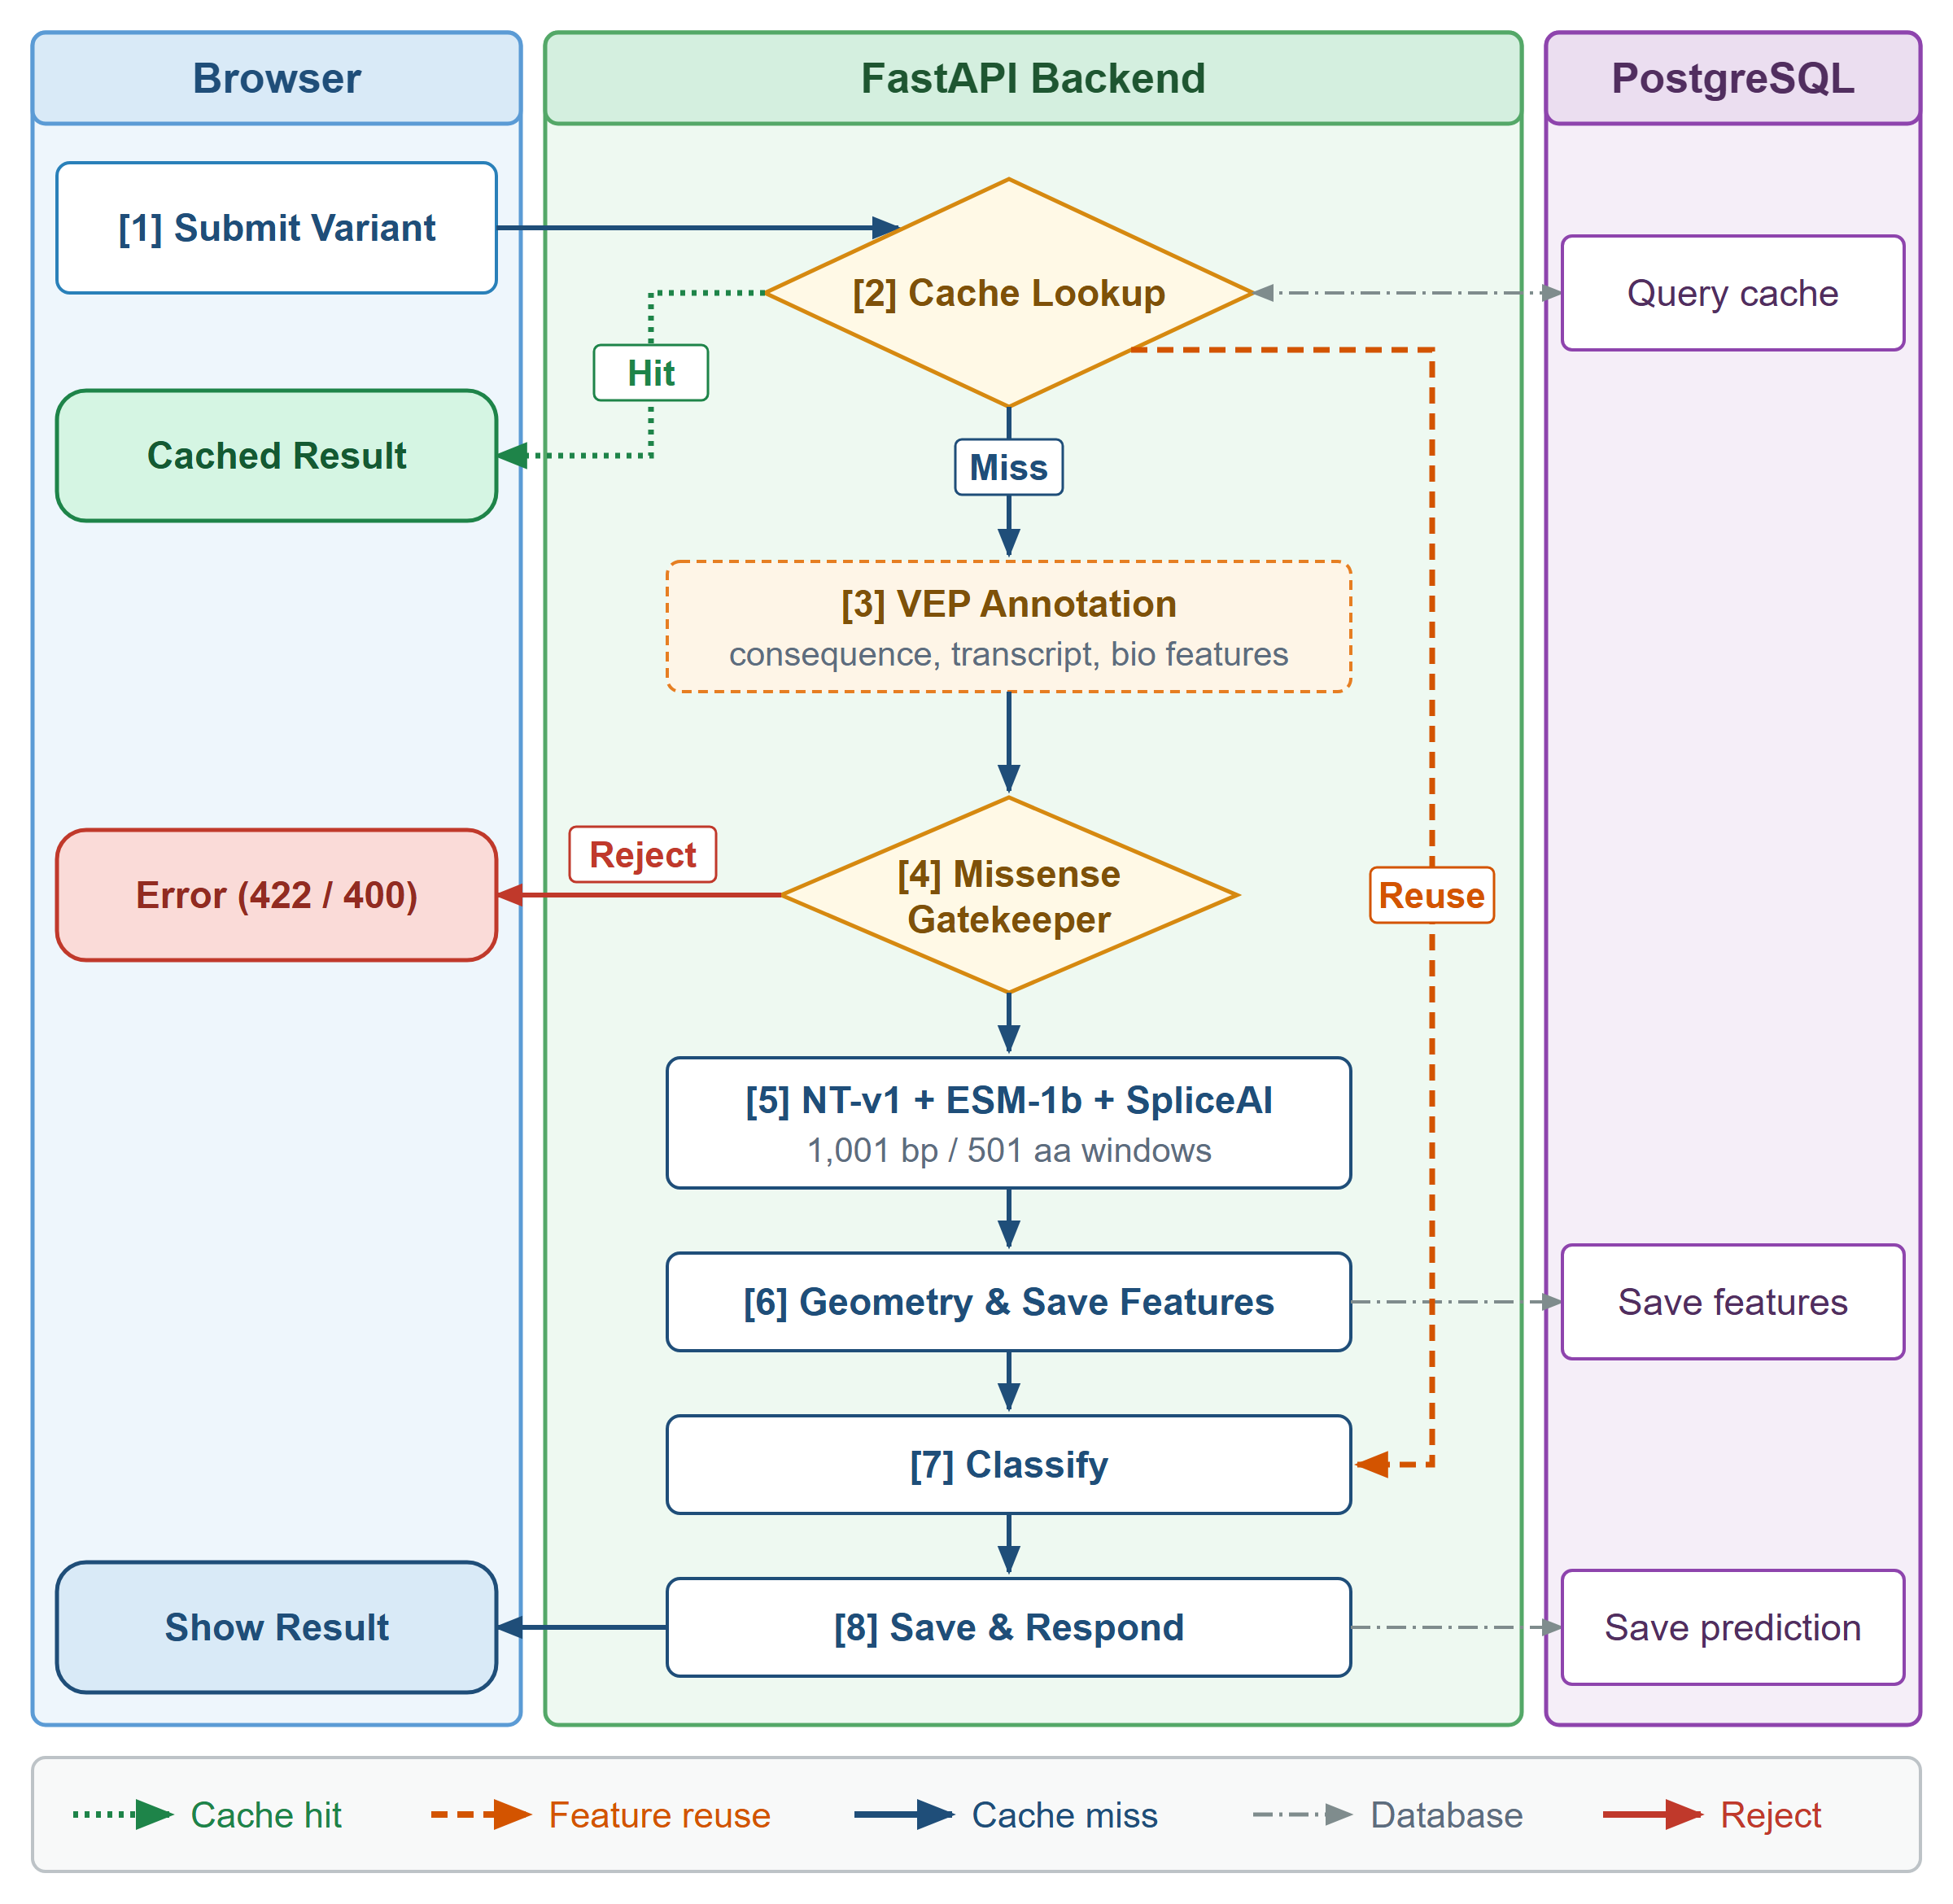
\includegraphics[width=0.95\textwidth]{figures/5.2.png}
    \caption{Single-variant inference workflow with hybrid lazy-caching.}
    \label{fig:single_sequence}
\end{figure}

\subsection{Batch Screening via Server-Sent Events}

Batch screening (Fig.~\ref{fig:batch_sse}) accepts a variant file (VCF, CSV, TXT, Parquet, or Excel) or a built-in $10$-variant benchmark cohort and streams results through SSE, which avoids HTTP timeouts and shows progress in real time. Uploaded files are read with automatic detection of common column names, and duplicate variants are removed. The variants are then processed in chunks of $64$, and each chunk passes through three stages:

\begin{enumerate}
    \item \textit{Chunk annotation:} the uncached variants of the chunk are annotated in a single VEP run, which uses several processes, and SpliceAI scores are read for the variants that pass the missense gatekeeper. Because VEP and SpliceAI use only the CPU, the next chunk is already annotated while the GPU processes the current one.
    \item \textit{Micro-batched feature extraction:} accepted variants are encoded in micro-batches of up to eight variants per foundation model forward pass. A micro-batch that exceeds the available GPU memory is automatically split in half and run again.
    \item \textit{Classification and streaming:} each variant is classified individually, and its result is sent as soon as it is ready, so the result table in the browser is updated step by step instead of waiting for the whole file.
\end{enumerate}

Results therefore start to appear after the first chunk instead of after the whole file has been annotated. The stream uses five event types: the current stage of each chunk, a classified variant, a variant skipped by the gatekeeper or coordinate validation, completion of the run with final statistics, and a system-level error. A single invalid variant is therefore reported with the reason, and the rest of the file continues to run. When the user stops the screening or leaves the page, the connection is closed and the backend cancels all remaining work: the running VEP process is terminated inside its container and no further chunk is processed. While a screening is running, the interface asks for confirmation before the user leaves the page.

\begin{figure}[htbp]
    \centering
    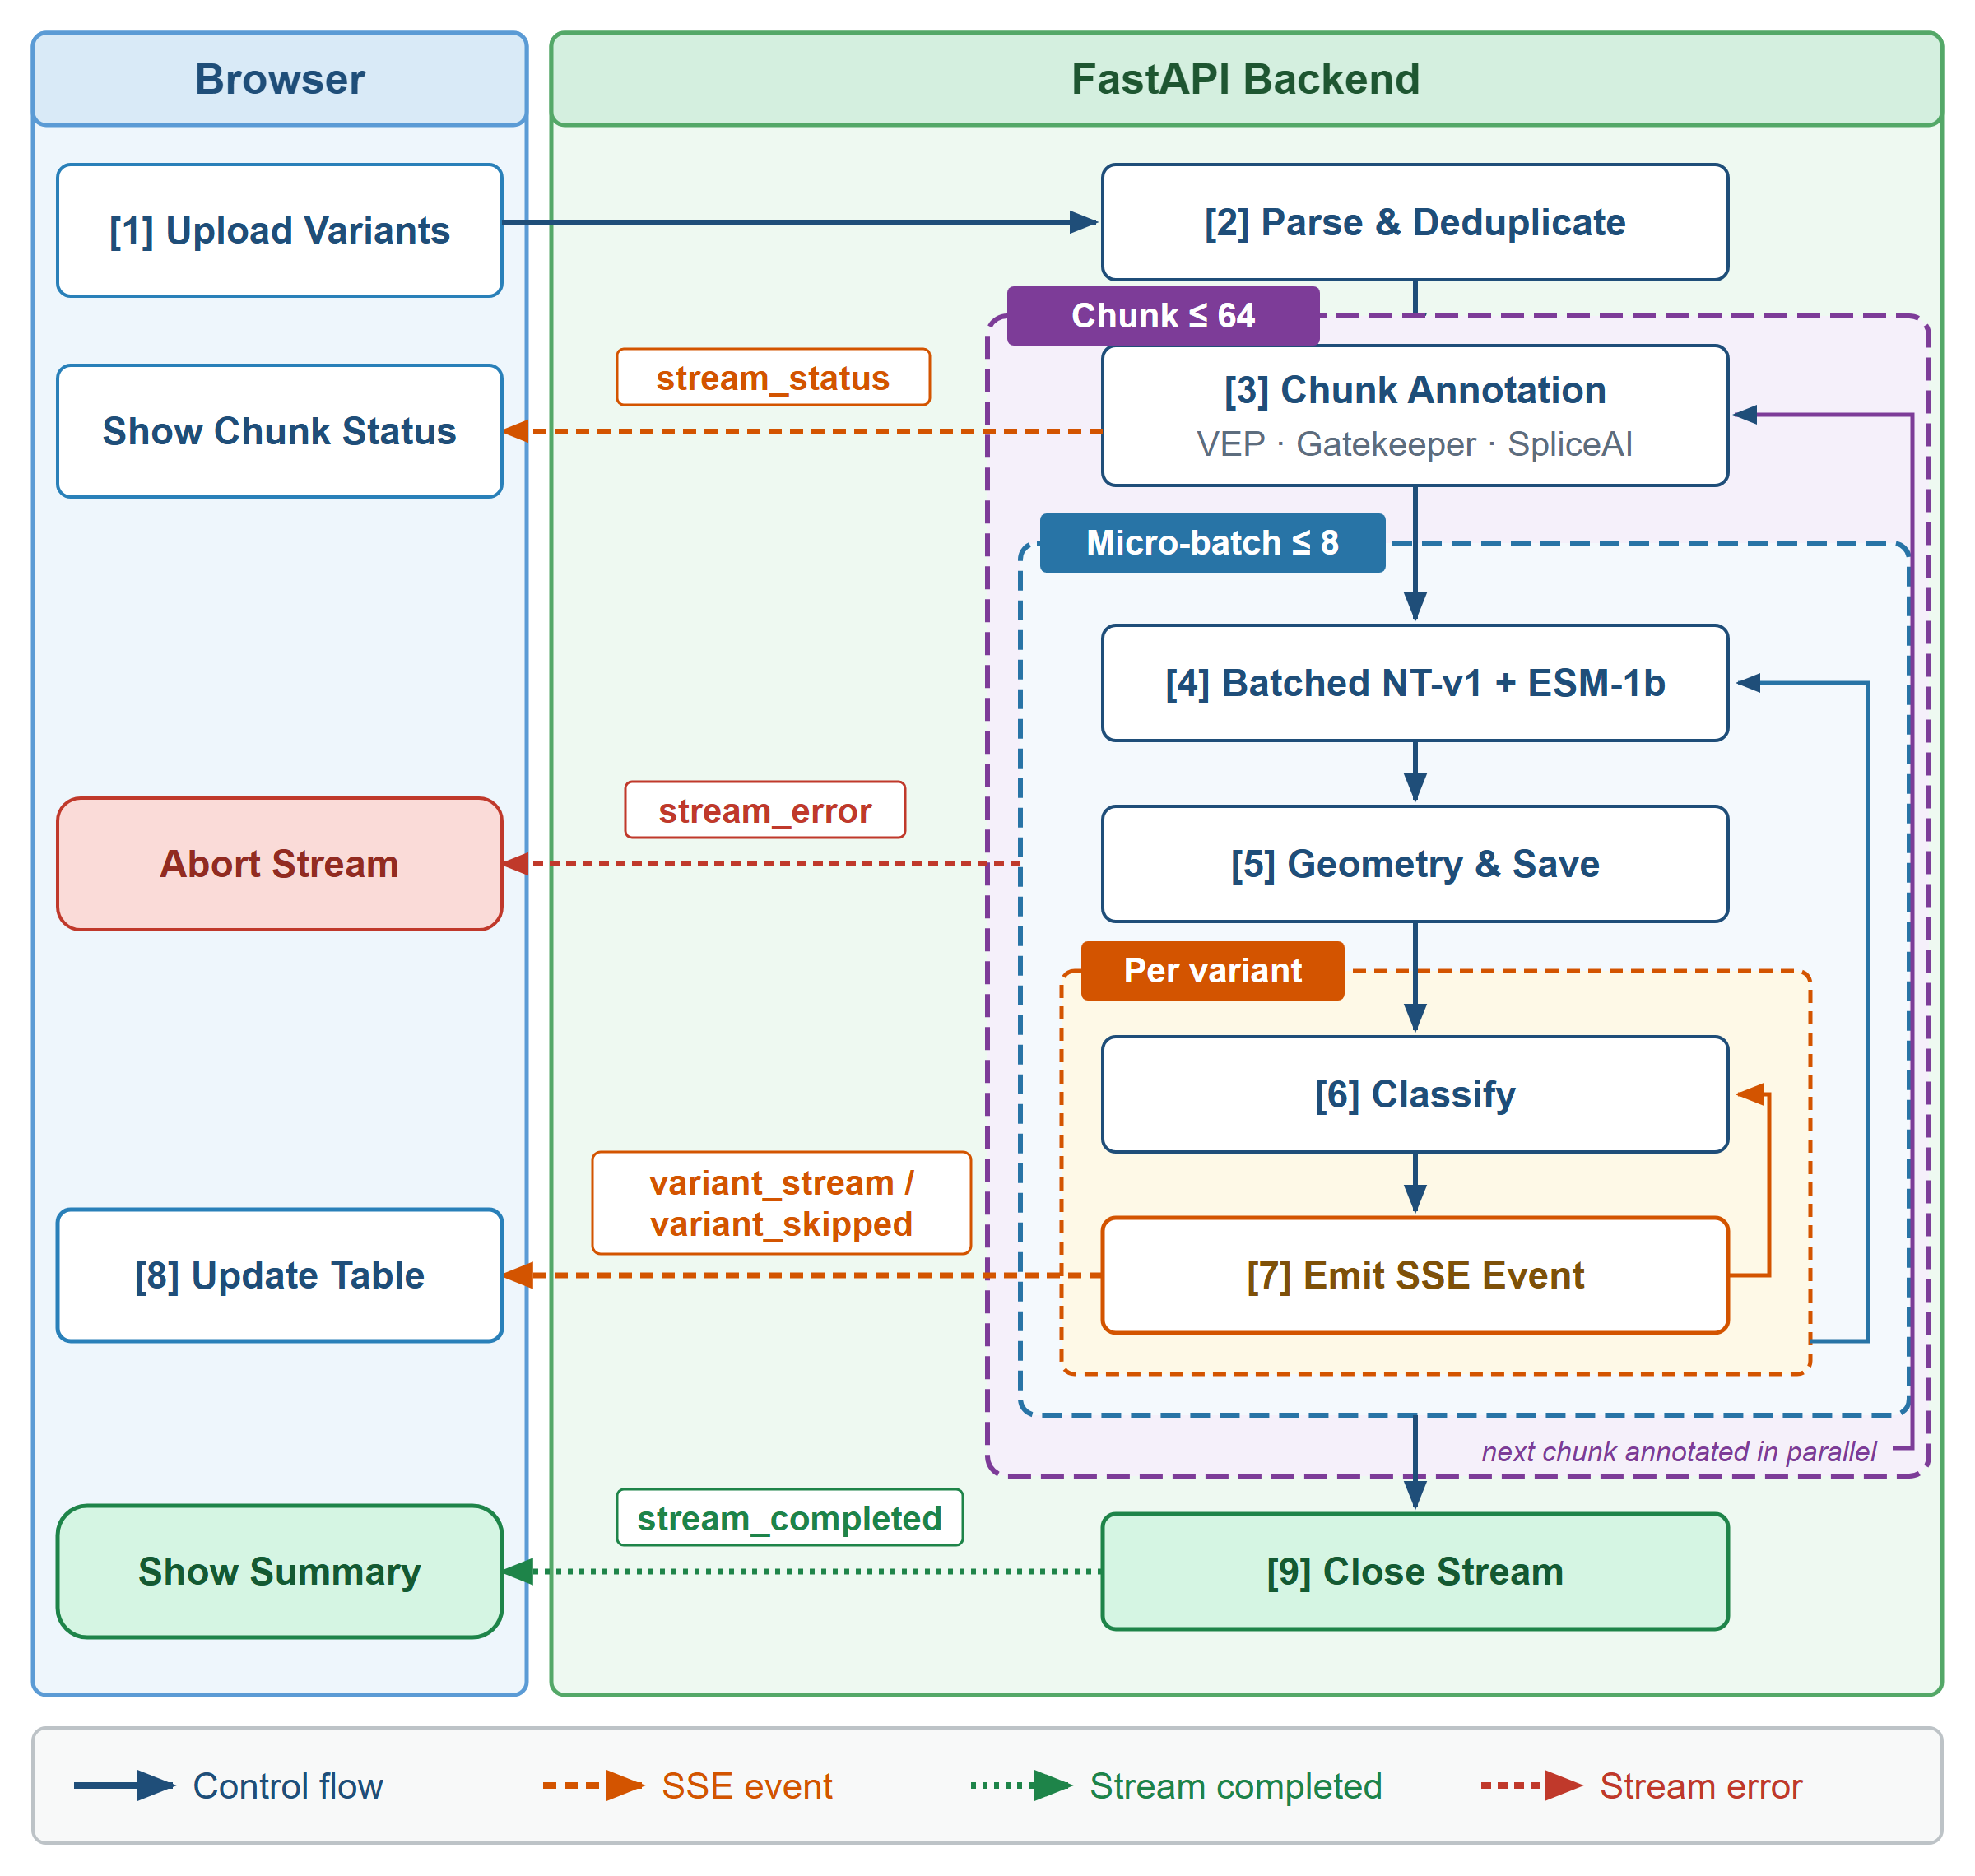
\includegraphics[width=0.95\textwidth]{figures/5.3.png}
    \caption{Batch screening workflow with chunked annotation, micro-batched inference, and SSE streaming.}
    \label{fig:batch_sse}
\end{figure}

% -------------------------------------------------------------------------------------
\section{Data Management and Deployment}
\label{sec:db_deployment}

The PostgreSQL database consists of three tables linked by foreign keys with cascading deletion (Table~\ref{tab:db_schema}). Separating features from predictions follows the caching strategy in Section~\ref{sec:data_flow}: one feature record is used for all seven configurations of a variant, and a unique index on the variant and configuration keeps at most one active prediction for each of them.

\begin{table}[htbp]
    \centering
    \caption{Main tables of the PostgreSQL database.}
    \label{tab:db_schema}
    \begin{tabular}{lp{0.22\textwidth}p{0.38\textwidth}}
        \toprule
        \textbf{Table} & \textbf{Number of records} & \textbf{Main contents} \\
        \midrule
        \texttt{variants} & One record per GRCh38 variant & Gene, consequence, protein change, and normalized ClinVar label \\
        \addlinespace
        \texttt{inference\_features} & One record per variant & DNA and protein token windows, four $1{,}280$-dimensional central-token embeddings, unscaled tabular features, VEP annotation, and hash of the extraction settings \\
        \addlinespace
        \texttt{predictions} & Up to seven records per variant & Probability, label, AlphaMissense and REVEL scores, Integrated Gradients attributions (added when first requested), and model version \\
        \bottomrule
    \end{tabular}
\end{table}

The token windows are stored in FP16 as binary columns and take about $0.34$~MB per variant, while the reference and alternative embeddings of the central token are stored as \texttt{pgvector} columns. The database only saves and loads these values, while nearest-neighbor search is performed by the FAISS indexes in memory. Tabular features are stored unscaled, so that normalization can be repeated without running the extraction again. All writes use the insert-or-update (upsert) operation of PostgreSQL, so requests that are repeated or sent at the same time update the existing record instead of creating duplicates.

The system uses a hybrid deployment: PostgreSQL and the offline VEP service run in Docker containers, which keeps their dependencies separate, while the FastAPI backend runs directly on the host machine to access the GPU through CUDA and loads the foundation models on the GPU only once at startup. The backend calls the VEP container locally, with the reference genome, VEP cache, and dbNSFP database mounted from the host, so no variant data are sent outside the workstation. A single startup script starts the database, backend, and frontend, while the VEP container is set up separately and must be running before annotation requests are sent. The main technologies are summarized in Table~\ref{tab:tech_stack}.

\begin{table}[htbp]
    \centering
    \caption{Technology stack of the TriMVPP system.}
    \label{tab:tech_stack}
    \begin{tabular}{ll}
        \toprule
        \textbf{Layer} & \textbf{Technologies} \\
        \midrule
        Frontend & React 19, TypeScript, Vite, Tailwind CSS, Recharts \\
        Backend & Python 3.10, FastAPI, Uvicorn, Pydantic, SQLAlchemy \\
        Deep learning & PyTorch 2.4 (CUDA 12.1), Hugging Face Transformers, FAISS \\
        Database & PostgreSQL 16 with \texttt{pgvector} (Docker) \\
        Bioinformatics & Ensembl VEP 116 with dbNSFP 5.3.1a (Docker), SpliceAI MANE v1.4, pyfaidx \\
        \bottomrule
    \end{tabular}
\end{table}

% -------------------------------------------------------------------------------------
\section{Web Interface}
\label{sec:web_interface}

The web interface (Fig.~\ref{fig:web_interface}) provides four views. The overview page (a) introduces the system and links to each module. The single-variant view (b) accepts a GRCh38 coordinate and the three feature switches, and displays the predicted probability and label together with ClinVar, AlphaMissense, and REVEL; the test-set MCC of the selected configuration is shown below the switches, and a \textit{Live Bypass} option makes the system compute the prediction again. The batch view (c) shows the streaming progress with the current chunk stage and the elapsed and estimated remaining time, the numbers of accepted and rejected variants, and a live table of the variants that are most likely to be pathogenic; all results can be exported as a CSV file. The explainability view (d) presents the Integrated Gradients attributions of a selected variant for each branch, token position, and tabular feature, together with the completeness error, and (e) the cross-attention maps, in which the user selects the query branch, layer, and head and can list the most-attended tokens of any query token. When a result is opened in another view, its variant and feature configuration are kept.

\begin{figure}[htbp]
    \centering
    \begin{minipage}{0.48\textwidth}\centering
        
\includegraphics[width=\linewidth]{figures/5.4a.png}\\[2pt]
        \small (a) System overview
    \end{minipage}\hfill
    \begin{minipage}{0.48\textwidth}\centering
        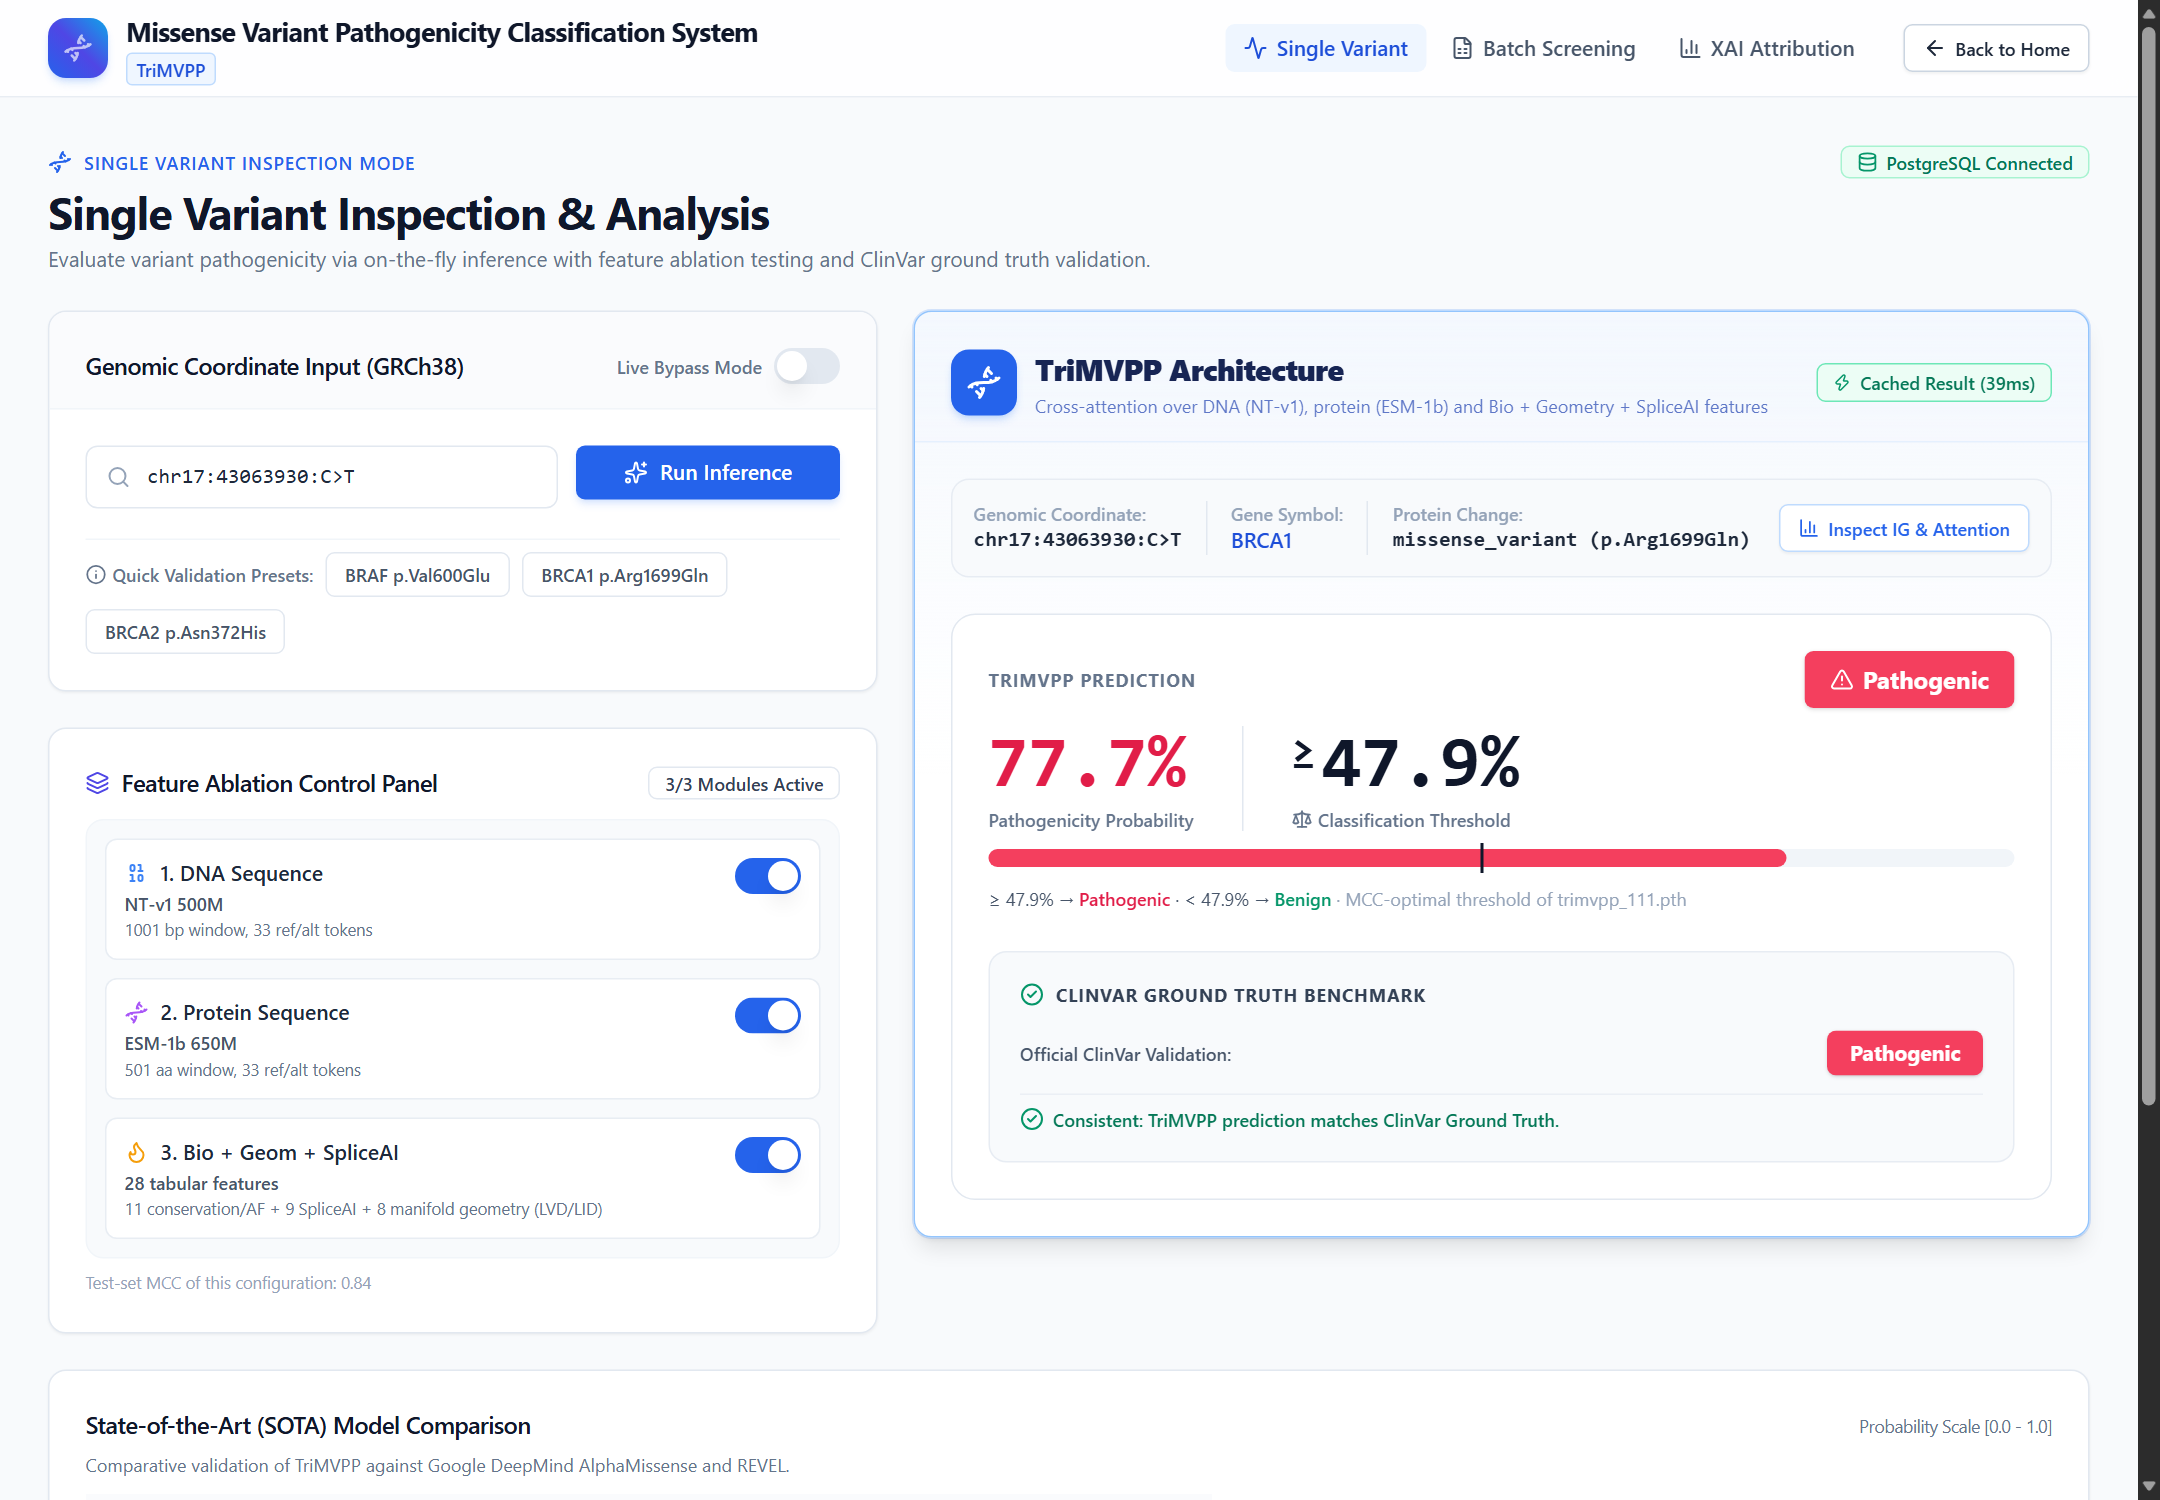
\includegraphics[width=\linewidth]{figures/5.4b.png}\\[2pt]
        \small (b) Single-variant inspection
    \end{minipage}\\[8pt]
    \begin{minipage}{0.48\textwidth}\centering
        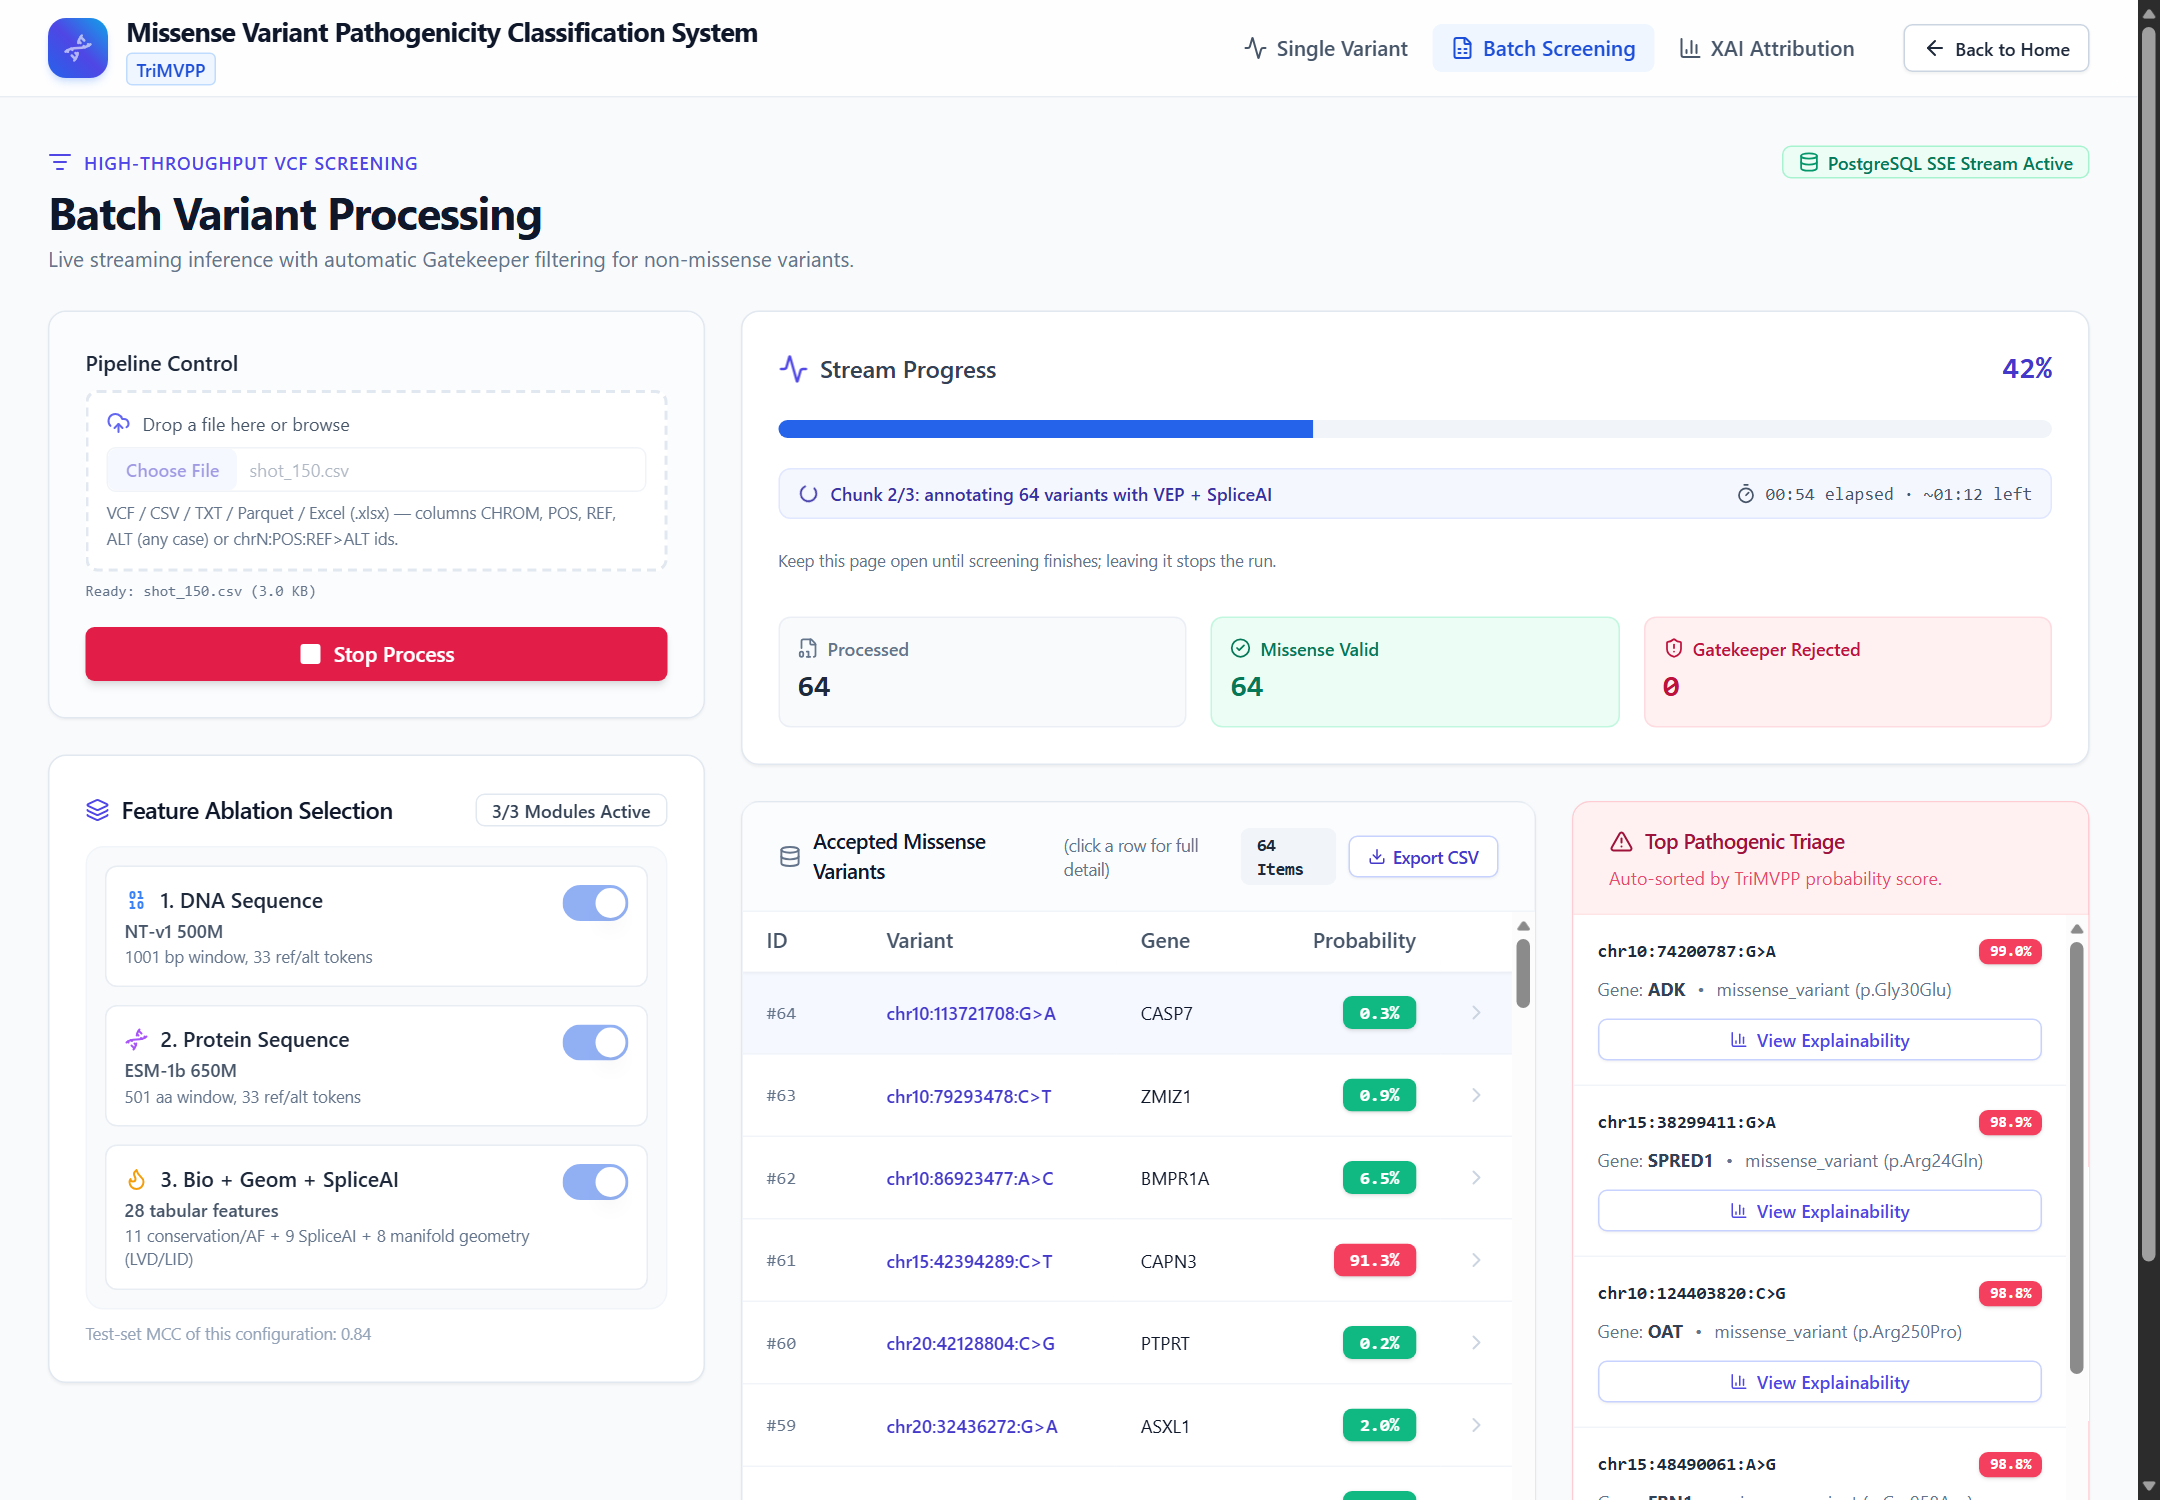
\includegraphics[width=\linewidth]{figures/5.4c.png}\\[2pt]
        \small (c) Batch screening
    \end{minipage}\hfill
    \begin{minipage}{0.48\textwidth}\centering
        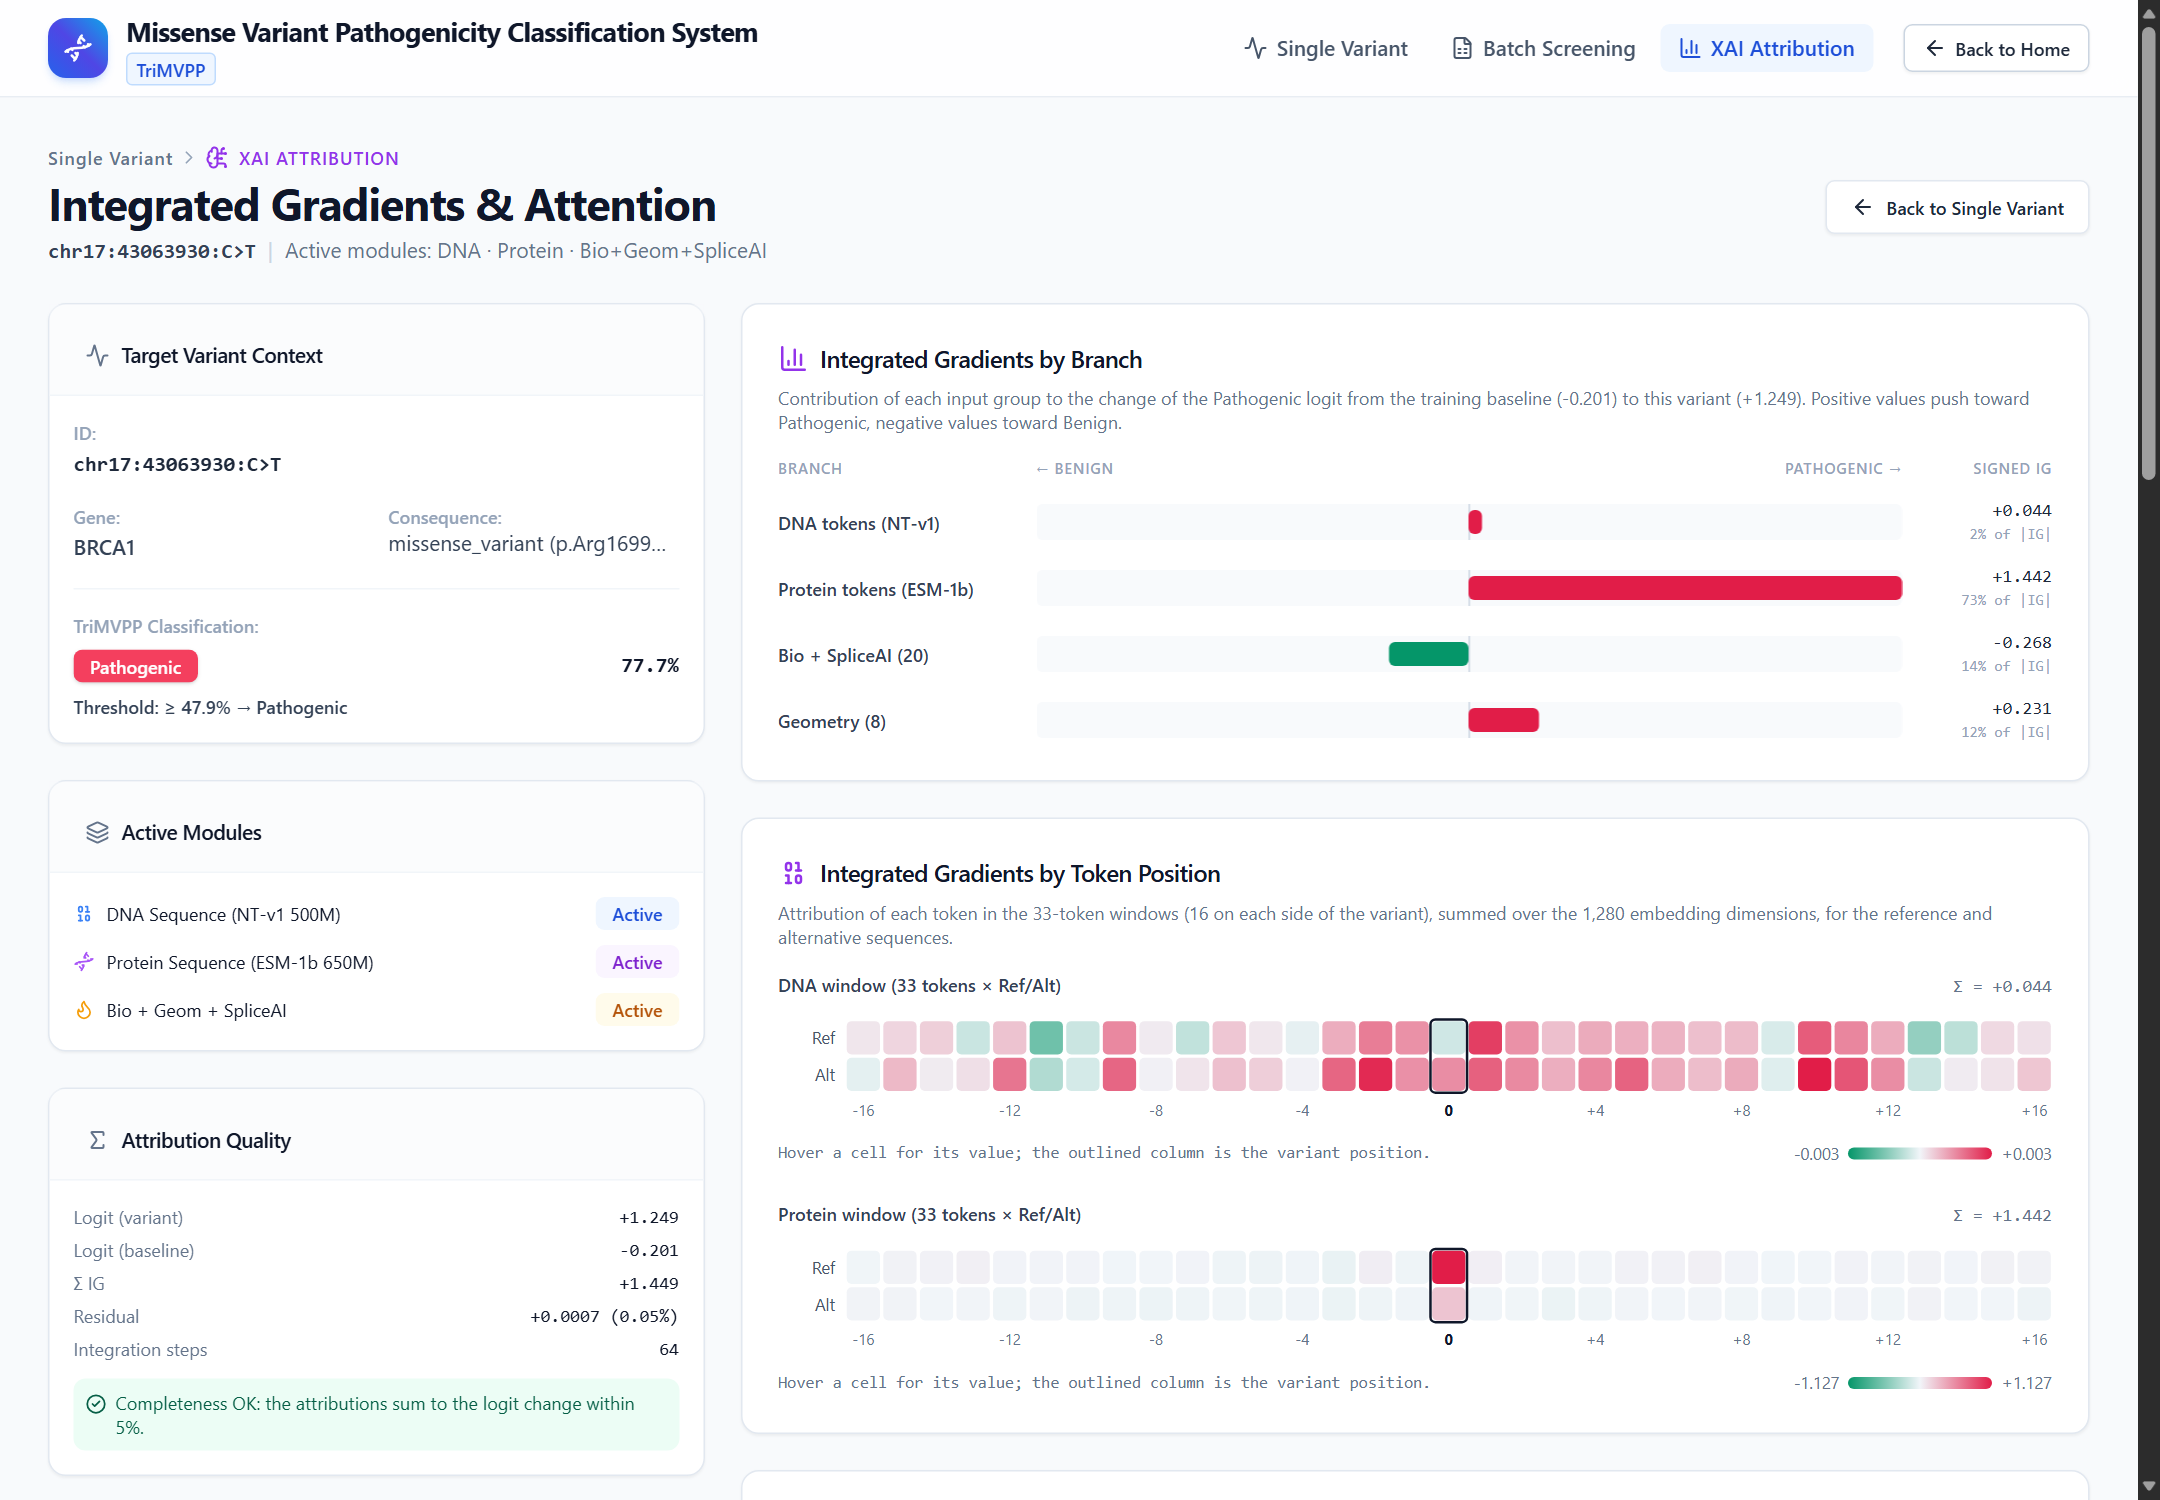
\includegraphics[width=\linewidth]{figures/5.4d.png}\\[2pt]
        \small (d) Integrated Gradients attributions
    \end{minipage}\\[8pt]
    \begin{minipage}{0.48\textwidth}\centering
        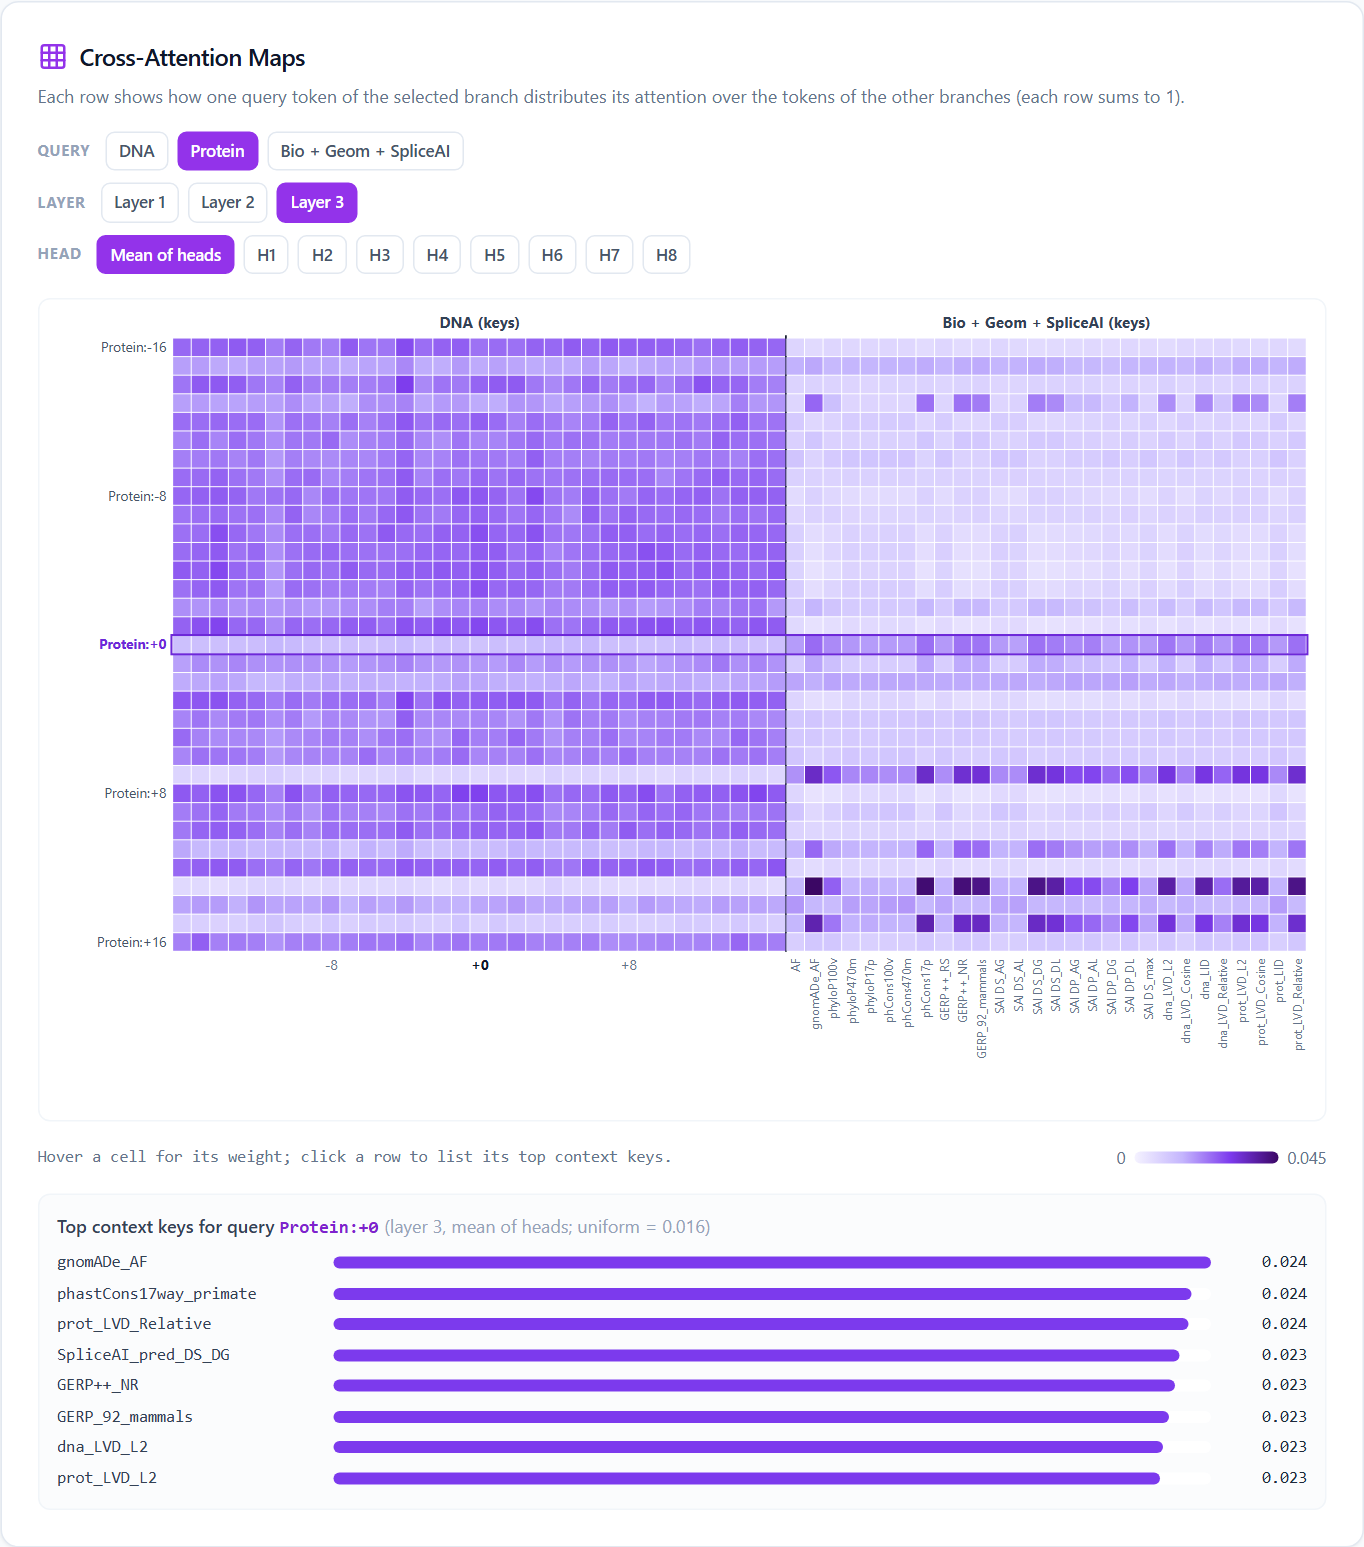
\includegraphics[width=\linewidth]{figures/5.4e.png}\\[2pt]
        \small (e) Cross-attention maps
    \end{minipage}
    \caption{Main views of the TriMVPP web interface.}
    \label{fig:web_interface}
\end{figure}

% -------------------------------------------------------------------------------------
\section{Latency Evaluation}
\label{sec:latency}

Latency was measured on a workstation with an AMD Ryzen~7 8745H CPU, 32~GB of RAM, and an NVIDIA GeForce RTX 4060 Laptop GPU (8~GB VRAM) running Windows~11, with all foundation models in FP16. Loading the models and reference resources at startup takes approximately $10$~s and $2.3$~GiB of GPU memory and is excluded from the measurements. Latency was recorded by the backend, from the time a request is received until the response is created, with one user sending requests one after another on the $10$-variant benchmark cohort (Table~\ref{tab:latency_benchmarks}). Each scenario was repeated three times over the cohort (ten times for cache hits) after a warm-up run, and the median is reported. For batch screening, the total is the time until the stream completes, and for the explainability view the time until the response is received, both measured by the client; the first opening of the explainability view was measured after the stored attributions had been removed. Feature reuse refers to the full configuration unless stated otherwise. Except for these two scenarios, the reported values therefore do not include JSON conversion and network transfer. None of them include browser display time, and they apply only to this hardware configuration.

\begin{table}[htbp]
    \centering
    \caption{Server-side processing latency across execution paths on the reference workstation.}
    \label{tab:latency_benchmarks}
    \begin{tabular}{p{0.33\textwidth}p{0.33\textwidth}r}
        \toprule
        \textbf{Scenario} & \textbf{Execution path} & \textbf{Latency} \\
        \midrule
        Single new variant & Full cache miss & 3.43 s / variant \\
        Batch cohort ($10$ variants) & Full cache miss & 8.6 s total \\
        Configuration change / Live Bypass & Feature reuse & 66 ms / query \\
        Repeated query & Full cache hit & 18 ms / query \\
        Explainability view, first opening & Cached prediction, IG + attention & 0.48 s / query \\
        Explainability view, later openings & Cached prediction and IG, attention & 0.14 s / query \\
        \bottomrule
    \end{tabular}
\end{table}

Batch processing reduces the average cost to $0.86$~s per variant, which is $4.0\times$ faster than sending single-variant requests one by one, mainly because VEP is run once per chunk and the foundation models process several variants per forward pass. For larger files, the overlap between the annotation of one chunk and the GPU processing of the previous one reduces the cost further: a file of $150$ new variants showed its first results after $29$~s and was completed in $72$~s ($0.48$~s per variant). For a new single variant, VEP annotation ($2.85$~s) accounts for about $83\%$ of the time, followed by the DNA and protein foundation models ($0.19$~s and $0.18$~s) and the SpliceAI lookup ($0.12$~s). Once a variant's features are stored, changing the configuration only repeats normalization and classification, which takes $66$~ms for the full configuration and $26$--$74$~ms for the other six. Because Integrated Gradients is computed only when needed, the first opening of the explainability view takes $0.48$~s for the full configuration, of which $0.29$~s is spent on Integrated Gradients, $0.30$~s for a two-branch configuration, and $0.10$~s for a single-branch one; later openings take $0.04$--$0.14$~s because the attributions are read from the database. Repeated queries are answered in $18$~ms, which is fast enough for interactive use.
